\documentclass[tikz,border=0pt]{standalone}
\usepackage{amsmath,newpxtext,newpxmath}
\begin{document}
% Created by tikzDevice version 0.12.6 on 2026-11-21 20:59:03
% !TEX encoding = UTF-8 Unicode
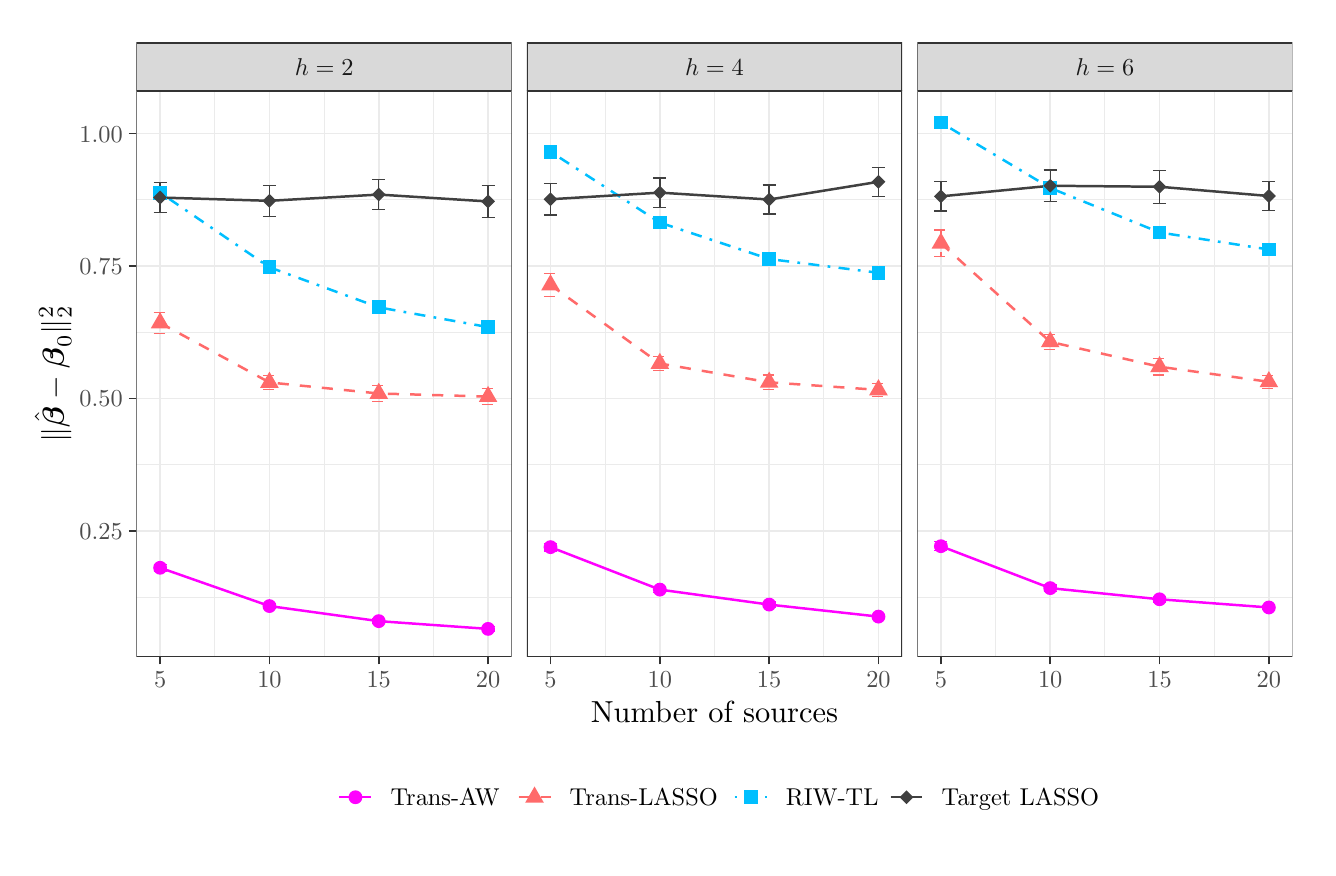
\begin{tikzpicture}[x=1pt,y=1pt]
\definecolor{fillColor}{RGB}{255,255,255}
\path[use as bounding box,fill=fillColor,fill opacity=0.00] (0,0) rectangle (462.53,296.31);
\begin{scope}
\path[clip] (  0.00,  0.00) rectangle (462.53,296.31);
\definecolor{drawColor}{RGB}{255,255,255}
\definecolor{fillColor}{RGB}{255,255,255}

\path[draw=drawColor,line width= 0.6pt,line join=round,line cap=round,fill=fillColor] (  0.00,  0.00) rectangle (462.53,296.31);
\end{scope}
\begin{scope}
\path[clip] ( 39.32, 68.96) rectangle (174.89,273.43);
\definecolor{fillColor}{RGB}{255,255,255}

\path[fill=fillColor] ( 39.32, 68.96) rectangle (174.89,273.43);
\definecolor{drawColor}{gray}{0.92}

\path[draw=drawColor,line width= 0.3pt,line join=round] ( 39.32, 90.53) --
	(174.89, 90.53);

\path[draw=drawColor,line width= 0.3pt,line join=round] ( 39.32,138.39) --
	(174.89,138.39);

\path[draw=drawColor,line width= 0.3pt,line join=round] ( 39.32,186.25) --
	(174.89,186.25);

\path[draw=drawColor,line width= 0.3pt,line join=round] ( 39.32,234.10) --
	(174.89,234.10);

\path[draw=drawColor,line width= 0.3pt,line join=round] ( 67.61, 68.96) --
	( 67.61,273.43);

\path[draw=drawColor,line width= 0.3pt,line join=round] (107.11, 68.96) --
	(107.11,273.43);

\path[draw=drawColor,line width= 0.3pt,line join=round] (146.61, 68.96) --
	(146.61,273.43);

\path[draw=drawColor,line width= 0.6pt,line join=round] ( 39.32,114.46) --
	(174.89,114.46);

\path[draw=drawColor,line width= 0.6pt,line join=round] ( 39.32,162.32) --
	(174.89,162.32);

\path[draw=drawColor,line width= 0.6pt,line join=round] ( 39.32,210.17) --
	(174.89,210.17);

\path[draw=drawColor,line width= 0.6pt,line join=round] ( 39.32,258.03) --
	(174.89,258.03);

\path[draw=drawColor,line width= 0.6pt,line join=round] ( 47.86, 68.96) --
	( 47.86,273.43);

\path[draw=drawColor,line width= 0.6pt,line join=round] ( 87.36, 68.96) --
	( 87.36,273.43);

\path[draw=drawColor,line width= 0.6pt,line join=round] (126.86, 68.96) --
	(126.86,273.43);

\path[draw=drawColor,line width= 0.6pt,line join=round] (166.36, 68.96) --
	(166.36,273.43);
\definecolor{drawColor}{RGB}{0,191,255}

\path[draw=drawColor,line width= 0.5pt,dash pattern=on 1pt off 3pt on 4pt off 3pt ,line join=round] ( 45.49,238.70) --
	( 50.23,238.70);

\path[draw=drawColor,line width= 0.5pt,dash pattern=on 1pt off 3pt on 4pt off 3pt ,line join=round] ( 47.86,238.70) --
	( 47.86,234.69);

\path[draw=drawColor,line width= 0.5pt,dash pattern=on 1pt off 3pt on 4pt off 3pt ,line join=round] ( 45.49,234.69) --
	( 50.23,234.69);

\path[draw=drawColor,line width= 0.5pt,dash pattern=on 1pt off 3pt on 4pt off 3pt ,line join=round] ( 84.99,211.14) --
	( 89.73,211.14);

\path[draw=drawColor,line width= 0.5pt,dash pattern=on 1pt off 3pt on 4pt off 3pt ,line join=round] ( 87.36,211.14) --
	( 87.36,208.33);

\path[draw=drawColor,line width= 0.5pt,dash pattern=on 1pt off 3pt on 4pt off 3pt ,line join=round] ( 84.99,208.33) --
	( 89.73,208.33);

\path[draw=drawColor,line width= 0.5pt,dash pattern=on 1pt off 3pt on 4pt off 3pt ,line join=round] (124.49,196.43) --
	(129.23,196.43);

\path[draw=drawColor,line width= 0.5pt,dash pattern=on 1pt off 3pt on 4pt off 3pt ,line join=round] (126.86,196.43) --
	(126.86,194.06);

\path[draw=drawColor,line width= 0.5pt,dash pattern=on 1pt off 3pt on 4pt off 3pt ,line join=round] (124.49,194.06) --
	(129.23,194.06);

\path[draw=drawColor,line width= 0.5pt,dash pattern=on 1pt off 3pt on 4pt off 3pt ,line join=round] (163.99,189.19) --
	(168.73,189.19);

\path[draw=drawColor,line width= 0.5pt,dash pattern=on 1pt off 3pt on 4pt off 3pt ,line join=round] (166.36,189.19) --
	(166.36,187.04);

\path[draw=drawColor,line width= 0.5pt,dash pattern=on 1pt off 3pt on 4pt off 3pt ,line join=round] (163.99,187.04) --
	(168.73,187.04);
\definecolor{drawColor}{gray}{0.25}

\path[draw=drawColor,line width= 0.5pt,line join=round] ( 45.49,240.30) --
	( 50.23,240.30);

\path[draw=drawColor,line width= 0.5pt,line join=round] ( 47.86,240.30) --
	( 47.86,229.56);

\path[draw=drawColor,line width= 0.5pt,line join=round] ( 45.49,229.56) --
	( 50.23,229.56);

\path[draw=drawColor,line width= 0.5pt,line join=round] ( 84.99,239.33) --
	( 89.73,239.33);

\path[draw=drawColor,line width= 0.5pt,line join=round] ( 87.36,239.33) --
	( 87.36,228.16);

\path[draw=drawColor,line width= 0.5pt,line join=round] ( 84.99,228.16) --
	( 89.73,228.16);

\path[draw=drawColor,line width= 0.5pt,line join=round] (124.49,241.41) --
	(129.23,241.41);

\path[draw=drawColor,line width= 0.5pt,line join=round] (126.86,241.41) --
	(126.86,230.59);

\path[draw=drawColor,line width= 0.5pt,line join=round] (124.49,230.59) --
	(129.23,230.59);

\path[draw=drawColor,line width= 0.5pt,line join=round] (163.99,239.37) --
	(168.73,239.37);

\path[draw=drawColor,line width= 0.5pt,line join=round] (166.36,239.37) --
	(166.36,227.65);

\path[draw=drawColor,line width= 0.5pt,line join=round] (163.99,227.65) --
	(168.73,227.65);
\definecolor{drawColor}{RGB}{255,0,255}

\path[draw=drawColor,line width= 0.5pt,line join=round] ( 45.49,102.42) --
	( 50.23,102.42);

\path[draw=drawColor,line width= 0.5pt,line join=round] ( 47.86,102.42) --
	( 47.86, 99.86);

\path[draw=drawColor,line width= 0.5pt,line join=round] ( 45.49, 99.86) --
	( 50.23, 99.86);

\path[draw=drawColor,line width= 0.5pt,line join=round] ( 84.99, 88.15) --
	( 89.73, 88.15);

\path[draw=drawColor,line width= 0.5pt,line join=round] ( 87.36, 88.15) --
	( 87.36, 86.47);

\path[draw=drawColor,line width= 0.5pt,line join=round] ( 84.99, 86.47) --
	( 89.73, 86.47);

\path[draw=drawColor,line width= 0.5pt,line join=round] (124.49, 82.61) --
	(129.23, 82.61);

\path[draw=drawColor,line width= 0.5pt,line join=round] (126.86, 82.61) --
	(126.86, 81.10);

\path[draw=drawColor,line width= 0.5pt,line join=round] (124.49, 81.10) --
	(129.23, 81.10);

\path[draw=drawColor,line width= 0.5pt,line join=round] (163.99, 79.88) --
	(168.73, 79.88);

\path[draw=drawColor,line width= 0.5pt,line join=round] (166.36, 79.88) --
	(166.36, 78.25);

\path[draw=drawColor,line width= 0.5pt,line join=round] (163.99, 78.25) --
	(168.73, 78.25);
\definecolor{drawColor}{RGB}{255,106,106}

\path[draw=drawColor,line width= 0.5pt,dash pattern=on 4pt off 4pt ,line join=round] ( 45.49,193.43) --
	( 50.23,193.43);

\path[draw=drawColor,line width= 0.5pt,dash pattern=on 4pt off 4pt ,line join=round] ( 47.86,193.43) --
	( 47.86,185.82);

\path[draw=drawColor,line width= 0.5pt,dash pattern=on 4pt off 4pt ,line join=round] ( 45.49,185.82) --
	( 50.23,185.82);

\path[draw=drawColor,line width= 0.5pt,dash pattern=on 4pt off 4pt ,line join=round] ( 84.99,170.56) --
	( 89.73,170.56);

\path[draw=drawColor,line width= 0.5pt,dash pattern=on 4pt off 4pt ,line join=round] ( 87.36,170.56) --
	( 87.36,165.67);

\path[draw=drawColor,line width= 0.5pt,dash pattern=on 4pt off 4pt ,line join=round] ( 84.99,165.67) --
	( 89.73,165.67);

\path[draw=drawColor,line width= 0.5pt,dash pattern=on 4pt off 4pt ,line join=round] (124.49,166.92) --
	(129.23,166.92);

\path[draw=drawColor,line width= 0.5pt,dash pattern=on 4pt off 4pt ,line join=round] (126.86,166.92) --
	(126.86,161.32);

\path[draw=drawColor,line width= 0.5pt,dash pattern=on 4pt off 4pt ,line join=round] (124.49,161.32) --
	(129.23,161.32);

\path[draw=drawColor,line width= 0.5pt,dash pattern=on 4pt off 4pt ,line join=round] (163.99,165.82) --
	(168.73,165.82);

\path[draw=drawColor,line width= 0.5pt,dash pattern=on 4pt off 4pt ,line join=round] (166.36,165.82) --
	(166.36,160.18);

\path[draw=drawColor,line width= 0.5pt,dash pattern=on 4pt off 4pt ,line join=round] (163.99,160.18) --
	(168.73,160.18);
\definecolor{drawColor}{RGB}{255,0,255}

\path[draw=drawColor,line width= 0.9pt,line join=round] ( 47.86,101.14) --
	( 87.36, 87.31) --
	(126.86, 81.86) --
	(166.36, 79.06);
\definecolor{drawColor}{RGB}{255,106,106}

\path[draw=drawColor,line width= 0.9pt,dash pattern=on 4pt off 4pt ,line join=round] ( 47.86,189.63) --
	( 87.36,168.11) --
	(126.86,164.12) --
	(166.36,163.00);
\definecolor{drawColor}{RGB}{0,191,255}

\path[draw=drawColor,line width= 0.9pt,dash pattern=on 1pt off 3pt on 4pt off 3pt ,line join=round] ( 47.86,236.69) --
	( 87.36,209.73) --
	(126.86,195.25) --
	(166.36,188.11);
\definecolor{drawColor}{gray}{0.25}

\path[draw=drawColor,line width= 0.9pt,line join=round] ( 47.86,234.93) --
	( 87.36,233.74) --
	(126.86,236.00) --
	(166.36,233.51);
\definecolor{fillColor}{RGB}{0,191,255}

\path[fill=fillColor] ( 45.36,234.19) --
	( 50.35,234.19) --
	( 50.35,239.19) --
	( 45.36,239.19) --
	cycle;

\path[fill=fillColor] ( 84.86,207.24) --
	( 89.86,207.24) --
	( 89.86,212.23) --
	( 84.86,212.23) --
	cycle;

\path[fill=fillColor] (124.36,192.75) --
	(129.36,192.75) --
	(129.36,197.75) --
	(124.36,197.75) --
	cycle;

\path[fill=fillColor] (163.86,185.62) --
	(168.86,185.62) --
	(168.86,190.61) --
	(163.86,190.61) --
	cycle;
\definecolor{fillColor}{gray}{0.25}

\path[fill=fillColor] ( 45.36,234.93) --
	( 47.86,237.43) --
	( 50.35,234.93) --
	( 47.86,232.44) --
	cycle;

\path[fill=fillColor] ( 84.86,233.74) --
	( 87.36,236.24) --
	( 89.86,233.74) --
	( 87.36,231.24) --
	cycle;

\path[fill=fillColor] (124.36,236.00) --
	(126.86,238.49) --
	(129.36,236.00) --
	(126.86,233.50) --
	cycle;

\path[fill=fillColor] (163.86,233.51) --
	(166.36,236.01) --
	(168.86,233.51) --
	(166.36,231.01) --
	cycle;
\definecolor{fillColor}{RGB}{255,0,255}

\path[fill=fillColor] ( 47.86,101.14) circle (  2.50);

\path[fill=fillColor] ( 87.36, 87.31) circle (  2.50);

\path[fill=fillColor] (126.86, 81.86) circle (  2.50);

\path[fill=fillColor] (166.36, 79.06) circle (  2.50);
\definecolor{fillColor}{RGB}{255,106,106}

\path[fill=fillColor] ( 47.86,193.51) --
	( 51.22,187.68) --
	( 44.49,187.68) --
	cycle;

\path[fill=fillColor] ( 87.36,172.00) --
	( 90.72,166.17) --
	( 83.99,166.17) --
	cycle;

\path[fill=fillColor] (126.86,168.00) --
	(130.22,162.18) --
	(123.50,162.18) --
	cycle;

\path[fill=fillColor] (166.36,166.88) --
	(169.72,161.06) --
	(163.00,161.06) --
	cycle;
\definecolor{drawColor}{gray}{0.20}

\path[draw=drawColor,line width= 0.6pt,line join=round,line cap=round] ( 39.32, 68.96) rectangle (174.89,273.43);
\end{scope}
\begin{scope}
\path[clip] (180.39, 68.96) rectangle (315.96,273.43);
\definecolor{fillColor}{RGB}{255,255,255}

\path[fill=fillColor] (180.39, 68.96) rectangle (315.96,273.43);
\definecolor{drawColor}{gray}{0.92}

\path[draw=drawColor,line width= 0.3pt,line join=round] (180.39, 90.53) --
	(315.96, 90.53);

\path[draw=drawColor,line width= 0.3pt,line join=round] (180.39,138.39) --
	(315.96,138.39);

\path[draw=drawColor,line width= 0.3pt,line join=round] (180.39,186.25) --
	(315.96,186.25);

\path[draw=drawColor,line width= 0.3pt,line join=round] (180.39,234.10) --
	(315.96,234.10);

\path[draw=drawColor,line width= 0.3pt,line join=round] (208.68, 68.96) --
	(208.68,273.43);

\path[draw=drawColor,line width= 0.3pt,line join=round] (248.18, 68.96) --
	(248.18,273.43);

\path[draw=drawColor,line width= 0.3pt,line join=round] (287.68, 68.96) --
	(287.68,273.43);

\path[draw=drawColor,line width= 0.6pt,line join=round] (180.39,114.46) --
	(315.96,114.46);

\path[draw=drawColor,line width= 0.6pt,line join=round] (180.39,162.32) --
	(315.96,162.32);

\path[draw=drawColor,line width= 0.6pt,line join=round] (180.39,210.17) --
	(315.96,210.17);

\path[draw=drawColor,line width= 0.6pt,line join=round] (180.39,258.03) --
	(315.96,258.03);

\path[draw=drawColor,line width= 0.6pt,line join=round] (188.92, 68.96) --
	(188.92,273.43);

\path[draw=drawColor,line width= 0.6pt,line join=round] (228.43, 68.96) --
	(228.43,273.43);

\path[draw=drawColor,line width= 0.6pt,line join=round] (267.93, 68.96) --
	(267.93,273.43);

\path[draw=drawColor,line width= 0.6pt,line join=round] (307.43, 68.96) --
	(307.43,273.43);
\definecolor{drawColor}{RGB}{0,191,255}

\path[draw=drawColor,line width= 0.5pt,dash pattern=on 1pt off 3pt on 4pt off 3pt ,line join=round] (186.55,253.41) --
	(191.29,253.41);

\path[draw=drawColor,line width= 0.5pt,dash pattern=on 1pt off 3pt on 4pt off 3pt ,line join=round] (188.92,253.41) --
	(188.92,249.57);

\path[draw=drawColor,line width= 0.5pt,dash pattern=on 1pt off 3pt on 4pt off 3pt ,line join=round] (186.55,249.57) --
	(191.29,249.57);

\path[draw=drawColor,line width= 0.5pt,dash pattern=on 1pt off 3pt on 4pt off 3pt ,line join=round] (226.06,227.55) --
	(230.80,227.55);

\path[draw=drawColor,line width= 0.5pt,dash pattern=on 1pt off 3pt on 4pt off 3pt ,line join=round] (228.43,227.55) --
	(228.43,224.21);

\path[draw=drawColor,line width= 0.5pt,dash pattern=on 1pt off 3pt on 4pt off 3pt ,line join=round] (226.06,224.21) --
	(230.80,224.21);

\path[draw=drawColor,line width= 0.5pt,dash pattern=on 1pt off 3pt on 4pt off 3pt ,line join=round] (265.56,214.14) --
	(270.30,214.14);

\path[draw=drawColor,line width= 0.5pt,dash pattern=on 1pt off 3pt on 4pt off 3pt ,line join=round] (267.93,214.14) --
	(267.93,211.28);

\path[draw=drawColor,line width= 0.5pt,dash pattern=on 1pt off 3pt on 4pt off 3pt ,line join=round] (265.56,211.28) --
	(270.30,211.28);

\path[draw=drawColor,line width= 0.5pt,dash pattern=on 1pt off 3pt on 4pt off 3pt ,line join=round] (305.06,209.03) --
	(309.80,209.03);

\path[draw=drawColor,line width= 0.5pt,dash pattern=on 1pt off 3pt on 4pt off 3pt ,line join=round] (307.43,209.03) --
	(307.43,206.45);

\path[draw=drawColor,line width= 0.5pt,dash pattern=on 1pt off 3pt on 4pt off 3pt ,line join=round] (305.06,206.45) --
	(309.80,206.45);
\definecolor{drawColor}{gray}{0.25}

\path[draw=drawColor,line width= 0.5pt,line join=round] (186.55,239.97) --
	(191.29,239.97);

\path[draw=drawColor,line width= 0.5pt,line join=round] (188.92,239.97) --
	(188.92,228.65);

\path[draw=drawColor,line width= 0.5pt,line join=round] (186.55,228.65) --
	(191.29,228.65);

\path[draw=drawColor,line width= 0.5pt,line join=round] (226.06,241.99) --
	(230.80,241.99);

\path[draw=drawColor,line width= 0.5pt,line join=round] (228.43,241.99) --
	(228.43,231.42);

\path[draw=drawColor,line width= 0.5pt,line join=round] (226.06,231.42) --
	(230.80,231.42);

\path[draw=drawColor,line width= 0.5pt,line join=round] (265.56,239.42) --
	(270.30,239.42);

\path[draw=drawColor,line width= 0.5pt,line join=round] (267.93,239.42) --
	(267.93,229.01);

\path[draw=drawColor,line width= 0.5pt,line join=round] (265.56,229.01) --
	(270.30,229.01);

\path[draw=drawColor,line width= 0.5pt,line join=round] (305.06,245.83) --
	(309.80,245.83);

\path[draw=drawColor,line width= 0.5pt,line join=round] (307.43,245.83) --
	(307.43,235.38);

\path[draw=drawColor,line width= 0.5pt,line join=round] (305.06,235.38) --
	(309.80,235.38);
\definecolor{drawColor}{RGB}{255,0,255}

\path[draw=drawColor,line width= 0.5pt,line join=round] (186.55,110.02) --
	(191.29,110.02);

\path[draw=drawColor,line width= 0.5pt,line join=round] (188.92,110.02) --
	(188.92,107.18);

\path[draw=drawColor,line width= 0.5pt,line join=round] (186.55,107.18) --
	(191.29,107.18);

\path[draw=drawColor,line width= 0.5pt,line join=round] (226.06, 94.28) --
	(230.80, 94.28);

\path[draw=drawColor,line width= 0.5pt,line join=round] (228.43, 94.28) --
	(228.43, 92.22);

\path[draw=drawColor,line width= 0.5pt,line join=round] (226.06, 92.22) --
	(230.80, 92.22);

\path[draw=drawColor,line width= 0.5pt,line join=round] (265.56, 88.71) --
	(270.30, 88.71);

\path[draw=drawColor,line width= 0.5pt,line join=round] (267.93, 88.71) --
	(267.93, 86.97);

\path[draw=drawColor,line width= 0.5pt,line join=round] (265.56, 86.97) --
	(270.30, 86.97);

\path[draw=drawColor,line width= 0.5pt,line join=round] (305.06, 84.19) --
	(309.80, 84.19);

\path[draw=drawColor,line width= 0.5pt,line join=round] (307.43, 84.19) --
	(307.43, 82.81);

\path[draw=drawColor,line width= 0.5pt,line join=round] (305.06, 82.81) --
	(309.80, 82.81);
\definecolor{drawColor}{RGB}{255,106,106}

\path[draw=drawColor,line width= 0.5pt,dash pattern=on 4pt off 4pt ,line join=round] (186.55,207.41) --
	(191.29,207.41);

\path[draw=drawColor,line width= 0.5pt,dash pattern=on 4pt off 4pt ,line join=round] (188.92,207.41) --
	(188.92,199.26);

\path[draw=drawColor,line width= 0.5pt,dash pattern=on 4pt off 4pt ,line join=round] (186.55,199.26) --
	(191.29,199.26);

\path[draw=drawColor,line width= 0.5pt,dash pattern=on 4pt off 4pt ,line join=round] (226.06,177.50) --
	(230.80,177.50);

\path[draw=drawColor,line width= 0.5pt,dash pattern=on 4pt off 4pt ,line join=round] (228.43,177.50) --
	(228.43,172.40);

\path[draw=drawColor,line width= 0.5pt,dash pattern=on 4pt off 4pt ,line join=round] (226.06,172.40) --
	(230.80,172.40);

\path[draw=drawColor,line width= 0.5pt,dash pattern=on 4pt off 4pt ,line join=round] (265.56,170.81) --
	(270.30,170.81);

\path[draw=drawColor,line width= 0.5pt,dash pattern=on 4pt off 4pt ,line join=round] (267.93,170.81) --
	(267.93,165.50);

\path[draw=drawColor,line width= 0.5pt,dash pattern=on 4pt off 4pt ,line join=round] (265.56,165.50) --
	(270.30,165.50);

\path[draw=drawColor,line width= 0.5pt,dash pattern=on 4pt off 4pt ,line join=round] (305.06,167.74) --
	(309.80,167.74);

\path[draw=drawColor,line width= 0.5pt,dash pattern=on 4pt off 4pt ,line join=round] (307.43,167.74) --
	(307.43,163.11);

\path[draw=drawColor,line width= 0.5pt,dash pattern=on 4pt off 4pt ,line join=round] (305.06,163.11) --
	(309.80,163.11);
\definecolor{drawColor}{RGB}{255,0,255}

\path[draw=drawColor,line width= 0.9pt,line join=round] (188.92,108.60) --
	(228.43, 93.25) --
	(267.93, 87.84) --
	(307.43, 83.50);
\definecolor{drawColor}{RGB}{255,106,106}

\path[draw=drawColor,line width= 0.9pt,dash pattern=on 4pt off 4pt ,line join=round] (188.92,203.33) --
	(228.43,174.95) --
	(267.93,168.16) --
	(307.43,165.42);
\definecolor{drawColor}{RGB}{0,191,255}

\path[draw=drawColor,line width= 0.9pt,dash pattern=on 1pt off 3pt on 4pt off 3pt ,line join=round] (188.92,251.49) --
	(228.43,225.88) --
	(267.93,212.71) --
	(307.43,207.74);
\definecolor{drawColor}{gray}{0.25}

\path[draw=drawColor,line width= 0.9pt,line join=round] (188.92,234.31) --
	(228.43,236.70) --
	(267.93,234.21) --
	(307.43,240.61);
\definecolor{fillColor}{RGB}{0,191,255}

\path[fill=fillColor] (186.43,248.99) --
	(191.42,248.99) --
	(191.42,253.99) --
	(186.43,253.99) --
	cycle;

\path[fill=fillColor] (225.93,223.38) --
	(230.92,223.38) --
	(230.92,228.38) --
	(225.93,228.38) --
	cycle;

\path[fill=fillColor] (265.43,210.21) --
	(270.42,210.21) --
	(270.42,215.21) --
	(265.43,215.21) --
	cycle;

\path[fill=fillColor] (304.93,205.24) --
	(309.93,205.24) --
	(309.93,210.24) --
	(304.93,210.24) --
	cycle;
\definecolor{fillColor}{gray}{0.25}

\path[fill=fillColor] (186.43,234.31) --
	(188.92,236.81) --
	(191.42,234.31) --
	(188.92,231.82) --
	cycle;

\path[fill=fillColor] (225.93,236.70) --
	(228.43,239.20) --
	(230.92,236.70) --
	(228.43,234.20) --
	cycle;

\path[fill=fillColor] (265.43,234.21) --
	(267.93,236.71) --
	(270.42,234.21) --
	(267.93,231.71) --
	cycle;

\path[fill=fillColor] (304.93,240.61) --
	(307.43,243.11) --
	(309.93,240.61) --
	(307.43,238.11) --
	cycle;
\definecolor{fillColor}{RGB}{255,0,255}

\path[fill=fillColor] (188.92,108.60) circle (  2.50);

\path[fill=fillColor] (228.43, 93.25) circle (  2.50);

\path[fill=fillColor] (267.93, 87.84) circle (  2.50);

\path[fill=fillColor] (307.43, 83.50) circle (  2.50);
\definecolor{fillColor}{RGB}{255,106,106}

\path[fill=fillColor] (188.92,207.22) --
	(192.29,201.39) --
	(185.56,201.39) --
	cycle;

\path[fill=fillColor] (228.43,178.84) --
	(231.79,173.01) --
	(225.06,173.01) --
	cycle;

\path[fill=fillColor] (267.93,172.04) --
	(271.29,166.21) --
	(264.56,166.21) --
	cycle;

\path[fill=fillColor] (307.43,169.31) --
	(310.79,163.48) --
	(304.06,163.48) --
	cycle;
\definecolor{drawColor}{gray}{0.20}

\path[draw=drawColor,line width= 0.6pt,line join=round,line cap=round] (180.39, 68.96) rectangle (315.96,273.43);
\end{scope}
\begin{scope}
\path[clip] (321.46, 68.96) rectangle (457.03,273.43);
\definecolor{fillColor}{RGB}{255,255,255}

\path[fill=fillColor] (321.46, 68.96) rectangle (457.03,273.43);
\definecolor{drawColor}{gray}{0.92}

\path[draw=drawColor,line width= 0.3pt,line join=round] (321.46, 90.53) --
	(457.03, 90.53);

\path[draw=drawColor,line width= 0.3pt,line join=round] (321.46,138.39) --
	(457.03,138.39);

\path[draw=drawColor,line width= 0.3pt,line join=round] (321.46,186.25) --
	(457.03,186.25);

\path[draw=drawColor,line width= 0.3pt,line join=round] (321.46,234.10) --
	(457.03,234.10);

\path[draw=drawColor,line width= 0.3pt,line join=round] (349.74, 68.96) --
	(349.74,273.43);

\path[draw=drawColor,line width= 0.3pt,line join=round] (389.24, 68.96) --
	(389.24,273.43);

\path[draw=drawColor,line width= 0.3pt,line join=round] (428.75, 68.96) --
	(428.75,273.43);

\path[draw=drawColor,line width= 0.6pt,line join=round] (321.46,114.46) --
	(457.03,114.46);

\path[draw=drawColor,line width= 0.6pt,line join=round] (321.46,162.32) --
	(457.03,162.32);

\path[draw=drawColor,line width= 0.6pt,line join=round] (321.46,210.17) --
	(457.03,210.17);

\path[draw=drawColor,line width= 0.6pt,line join=round] (321.46,258.03) --
	(457.03,258.03);

\path[draw=drawColor,line width= 0.6pt,line join=round] (329.99, 68.96) --
	(329.99,273.43);

\path[draw=drawColor,line width= 0.6pt,line join=round] (369.49, 68.96) --
	(369.49,273.43);

\path[draw=drawColor,line width= 0.6pt,line join=round] (408.99, 68.96) --
	(408.99,273.43);

\path[draw=drawColor,line width= 0.6pt,line join=round] (448.50, 68.96) --
	(448.50,273.43);
\definecolor{drawColor}{RGB}{0,191,255}

\path[draw=drawColor,line width= 0.5pt,dash pattern=on 1pt off 3pt on 4pt off 3pt ,line join=round] (327.62,264.13) --
	(332.36,264.13);

\path[draw=drawColor,line width= 0.5pt,dash pattern=on 1pt off 3pt on 4pt off 3pt ,line join=round] (329.99,264.13) --
	(329.99,259.90);

\path[draw=drawColor,line width= 0.5pt,dash pattern=on 1pt off 3pt on 4pt off 3pt ,line join=round] (327.62,259.90) --
	(332.36,259.90);

\path[draw=drawColor,line width= 0.5pt,dash pattern=on 1pt off 3pt on 4pt off 3pt ,line join=round] (367.12,240.33) --
	(371.86,240.33);

\path[draw=drawColor,line width= 0.5pt,dash pattern=on 1pt off 3pt on 4pt off 3pt ,line join=round] (369.49,240.33) --
	(369.49,236.46);

\path[draw=drawColor,line width= 0.5pt,dash pattern=on 1pt off 3pt on 4pt off 3pt ,line join=round] (367.12,236.46) --
	(371.86,236.46);

\path[draw=drawColor,line width= 0.5pt,dash pattern=on 1pt off 3pt on 4pt off 3pt ,line join=round] (406.62,224.07) --
	(411.36,224.07);

\path[draw=drawColor,line width= 0.5pt,dash pattern=on 1pt off 3pt on 4pt off 3pt ,line join=round] (408.99,224.07) --
	(408.99,220.57);

\path[draw=drawColor,line width= 0.5pt,dash pattern=on 1pt off 3pt on 4pt off 3pt ,line join=round] (406.62,220.57) --
	(411.36,220.57);

\path[draw=drawColor,line width= 0.5pt,dash pattern=on 1pt off 3pt on 4pt off 3pt ,line join=round] (446.13,217.71) --
	(450.87,217.71);

\path[draw=drawColor,line width= 0.5pt,dash pattern=on 1pt off 3pt on 4pt off 3pt ,line join=round] (448.50,217.71) --
	(448.50,214.57);

\path[draw=drawColor,line width= 0.5pt,dash pattern=on 1pt off 3pt on 4pt off 3pt ,line join=round] (446.13,214.57) --
	(450.87,214.57);
\definecolor{drawColor}{gray}{0.25}

\path[draw=drawColor,line width= 0.5pt,line join=round] (327.62,240.67) --
	(332.36,240.67);

\path[draw=drawColor,line width= 0.5pt,line join=round] (329.99,240.67) --
	(329.99,230.03);

\path[draw=drawColor,line width= 0.5pt,line join=round] (327.62,230.03) --
	(332.36,230.03);

\path[draw=drawColor,line width= 0.5pt,line join=round] (367.12,244.93) --
	(371.86,244.93);

\path[draw=drawColor,line width= 0.5pt,line join=round] (369.49,244.93) --
	(369.49,233.43);

\path[draw=drawColor,line width= 0.5pt,line join=round] (367.12,233.43) --
	(371.86,233.43);

\path[draw=drawColor,line width= 0.5pt,line join=round] (406.62,244.78) --
	(411.36,244.78);

\path[draw=drawColor,line width= 0.5pt,line join=round] (408.99,244.78) --
	(408.99,232.86);

\path[draw=drawColor,line width= 0.5pt,line join=round] (406.62,232.86) --
	(411.36,232.86);

\path[draw=drawColor,line width= 0.5pt,line join=round] (446.13,240.79) --
	(450.87,240.79);

\path[draw=drawColor,line width= 0.5pt,line join=round] (448.50,240.79) --
	(448.50,230.17);

\path[draw=drawColor,line width= 0.5pt,line join=round] (446.13,230.17) --
	(450.87,230.17);
\definecolor{drawColor}{RGB}{255,0,255}

\path[draw=drawColor,line width= 0.5pt,line join=round] (327.62,110.55) --
	(332.36,110.55);

\path[draw=drawColor,line width= 0.5pt,line join=round] (329.99,110.55) --
	(329.99,107.33);

\path[draw=drawColor,line width= 0.5pt,line join=round] (327.62,107.33) --
	(332.36,107.33);

\path[draw=drawColor,line width= 0.5pt,line join=round] (367.12, 94.92) --
	(371.86, 94.92);

\path[draw=drawColor,line width= 0.5pt,line join=round] (369.49, 94.92) --
	(369.49, 92.65);

\path[draw=drawColor,line width= 0.5pt,line join=round] (367.12, 92.65) --
	(371.86, 92.65);

\path[draw=drawColor,line width= 0.5pt,line join=round] (406.62, 90.71) --
	(411.36, 90.71);

\path[draw=drawColor,line width= 0.5pt,line join=round] (408.99, 90.71) --
	(408.99, 88.81);

\path[draw=drawColor,line width= 0.5pt,line join=round] (406.62, 88.81) --
	(411.36, 88.81);

\path[draw=drawColor,line width= 0.5pt,line join=round] (446.13, 87.61) --
	(450.87, 87.61);

\path[draw=drawColor,line width= 0.5pt,line join=round] (448.50, 87.61) --
	(448.50, 86.00);

\path[draw=drawColor,line width= 0.5pt,line join=round] (446.13, 86.00) --
	(450.87, 86.00);
\definecolor{drawColor}{RGB}{255,106,106}

\path[draw=drawColor,line width= 0.5pt,dash pattern=on 4pt off 4pt ,line join=round] (327.62,223.13) --
	(332.36,223.13);

\path[draw=drawColor,line width= 0.5pt,dash pattern=on 4pt off 4pt ,line join=round] (329.99,223.13) --
	(329.99,213.69);

\path[draw=drawColor,line width= 0.5pt,dash pattern=on 4pt off 4pt ,line join=round] (327.62,213.69) --
	(332.36,213.69);

\path[draw=drawColor,line width= 0.5pt,dash pattern=on 4pt off 4pt ,line join=round] (367.12,185.47) --
	(371.86,185.47);

\path[draw=drawColor,line width= 0.5pt,dash pattern=on 4pt off 4pt ,line join=round] (369.49,185.47) --
	(369.49,180.09);

\path[draw=drawColor,line width= 0.5pt,dash pattern=on 4pt off 4pt ,line join=round] (367.12,180.09) --
	(371.86,180.09);

\path[draw=drawColor,line width= 0.5pt,dash pattern=on 4pt off 4pt ,line join=round] (406.62,176.79) --
	(411.36,176.79);

\path[draw=drawColor,line width= 0.5pt,dash pattern=on 4pt off 4pt ,line join=round] (408.99,176.79) --
	(408.99,170.79);

\path[draw=drawColor,line width= 0.5pt,dash pattern=on 4pt off 4pt ,line join=round] (406.62,170.79) --
	(411.36,170.79);

\path[draw=drawColor,line width= 0.5pt,dash pattern=on 4pt off 4pt ,line join=round] (446.13,170.70) --
	(450.87,170.70);

\path[draw=drawColor,line width= 0.5pt,dash pattern=on 4pt off 4pt ,line join=round] (448.50,170.70) --
	(448.50,165.99);

\path[draw=drawColor,line width= 0.5pt,dash pattern=on 4pt off 4pt ,line join=round] (446.13,165.99) --
	(450.87,165.99);
\definecolor{drawColor}{RGB}{255,0,255}

\path[draw=drawColor,line width= 0.9pt,line join=round] (329.99,108.94) --
	(369.49, 93.79) --
	(408.99, 89.76) --
	(448.50, 86.80);
\definecolor{drawColor}{RGB}{255,106,106}

\path[draw=drawColor,line width= 0.9pt,dash pattern=on 4pt off 4pt ,line join=round] (329.99,218.41) --
	(369.49,182.78) --
	(408.99,173.79) --
	(448.50,168.34);
\definecolor{drawColor}{RGB}{0,191,255}

\path[draw=drawColor,line width= 0.9pt,dash pattern=on 1pt off 3pt on 4pt off 3pt ,line join=round] (329.99,262.01) --
	(369.49,238.39) --
	(408.99,222.32) --
	(448.50,216.14);
\definecolor{drawColor}{gray}{0.25}

\path[draw=drawColor,line width= 0.9pt,line join=round] (329.99,235.35) --
	(369.49,239.18) --
	(408.99,238.82) --
	(448.50,235.48);
\definecolor{fillColor}{RGB}{0,191,255}

\path[fill=fillColor] (327.49,259.52) --
	(332.49,259.52) --
	(332.49,264.51) --
	(327.49,264.51) --
	cycle;

\path[fill=fillColor] (367.00,235.90) --
	(371.99,235.90) --
	(371.99,240.89) --
	(367.00,240.89) --
	cycle;

\path[fill=fillColor] (406.50,219.82) --
	(411.49,219.82) --
	(411.49,224.82) --
	(406.50,224.82) --
	cycle;

\path[fill=fillColor] (446.00,213.64) --
	(450.99,213.64) --
	(450.99,218.64) --
	(446.00,218.64) --
	cycle;
\definecolor{fillColor}{gray}{0.25}

\path[fill=fillColor] (327.49,235.35) --
	(329.99,237.84) --
	(332.49,235.35) --
	(329.99,232.85) --
	cycle;

\path[fill=fillColor] (367.00,239.18) --
	(369.49,241.68) --
	(371.99,239.18) --
	(369.49,236.68) --
	cycle;

\path[fill=fillColor] (406.50,238.82) --
	(408.99,241.32) --
	(411.49,238.82) --
	(408.99,236.32) --
	cycle;

\path[fill=fillColor] (446.00,235.48) --
	(448.50,237.98) --
	(450.99,235.48) --
	(448.50,232.98) --
	cycle;
\definecolor{fillColor}{RGB}{255,0,255}

\path[fill=fillColor] (329.99,108.94) circle (  2.50);

\path[fill=fillColor] (369.49, 93.79) circle (  2.50);

\path[fill=fillColor] (408.99, 89.76) circle (  2.50);

\path[fill=fillColor] (448.50, 86.80) circle (  2.50);
\definecolor{fillColor}{RGB}{255,106,106}

\path[fill=fillColor] (329.99,222.29) --
	(333.36,216.47) --
	(326.63,216.47) --
	cycle;

\path[fill=fillColor] (369.49,186.67) --
	(372.86,180.84) --
	(366.13,180.84) --
	cycle;

\path[fill=fillColor] (408.99,177.67) --
	(412.36,171.85) --
	(405.63,171.85) --
	cycle;

\path[fill=fillColor] (448.50,172.23) --
	(451.86,166.40) --
	(445.13,166.40) --
	cycle;
\definecolor{drawColor}{gray}{0.20}

\path[draw=drawColor,line width= 0.6pt,line join=round,line cap=round] (321.46, 68.96) rectangle (457.03,273.43);
\end{scope}
\begin{scope}
\path[clip] ( 39.32,273.43) rectangle (174.89,290.81);
\definecolor{drawColor}{gray}{0.20}
\definecolor{fillColor}{gray}{0.85}

\path[draw=drawColor,line width= 0.6pt,line join=round,line cap=round,fill=fillColor] ( 39.32,273.43) rectangle (174.89,290.81);
\definecolor{drawColor}{gray}{0.10}

\node[text=drawColor,anchor=base,inner sep=0pt, outer sep=0pt, scale=  0.88] at (107.11,279.07) {$h = 2$};
\end{scope}
\begin{scope}
\path[clip] (180.39,273.43) rectangle (315.96,290.81);
\definecolor{drawColor}{gray}{0.20}
\definecolor{fillColor}{gray}{0.85}

\path[draw=drawColor,line width= 0.6pt,line join=round,line cap=round,fill=fillColor] (180.39,273.43) rectangle (315.96,290.81);
\definecolor{drawColor}{gray}{0.10}

\node[text=drawColor,anchor=base,inner sep=0pt, outer sep=0pt, scale=  0.88] at (248.18,279.07) {$h = 4$};
\end{scope}
\begin{scope}
\path[clip] (321.46,273.43) rectangle (457.03,290.81);
\definecolor{drawColor}{gray}{0.20}
\definecolor{fillColor}{gray}{0.85}

\path[draw=drawColor,line width= 0.6pt,line join=round,line cap=round,fill=fillColor] (321.46,273.43) rectangle (457.03,290.81);
\definecolor{drawColor}{gray}{0.10}

\node[text=drawColor,anchor=base,inner sep=0pt, outer sep=0pt, scale=  0.88] at (389.24,279.07) {$h = 6$};
\end{scope}
\begin{scope}
\path[clip] (  0.00,  0.00) rectangle (462.53,296.31);
\definecolor{drawColor}{gray}{0.20}

\path[draw=drawColor,line width= 0.6pt,line join=round] ( 47.86, 66.21) --
	( 47.86, 68.96);

\path[draw=drawColor,line width= 0.6pt,line join=round] ( 87.36, 66.21) --
	( 87.36, 68.96);

\path[draw=drawColor,line width= 0.6pt,line join=round] (126.86, 66.21) --
	(126.86, 68.96);

\path[draw=drawColor,line width= 0.6pt,line join=round] (166.36, 66.21) --
	(166.36, 68.96);
\end{scope}
\begin{scope}
\path[clip] (  0.00,  0.00) rectangle (462.53,296.31);
\definecolor{drawColor}{gray}{0.30}

\node[text=drawColor,anchor=base,inner sep=0pt, outer sep=0pt, scale=  0.88] at ( 47.86, 57.91) {5};

\node[text=drawColor,anchor=base,inner sep=0pt, outer sep=0pt, scale=  0.88] at ( 87.36, 57.91) {10};

\node[text=drawColor,anchor=base,inner sep=0pt, outer sep=0pt, scale=  0.88] at (126.86, 57.91) {15};

\node[text=drawColor,anchor=base,inner sep=0pt, outer sep=0pt, scale=  0.88] at (166.36, 57.91) {20};
\end{scope}
\begin{scope}
\path[clip] (  0.00,  0.00) rectangle (462.53,296.31);
\definecolor{drawColor}{gray}{0.20}

\path[draw=drawColor,line width= 0.6pt,line join=round] (188.92, 66.21) --
	(188.92, 68.96);

\path[draw=drawColor,line width= 0.6pt,line join=round] (228.43, 66.21) --
	(228.43, 68.96);

\path[draw=drawColor,line width= 0.6pt,line join=round] (267.93, 66.21) --
	(267.93, 68.96);

\path[draw=drawColor,line width= 0.6pt,line join=round] (307.43, 66.21) --
	(307.43, 68.96);
\end{scope}
\begin{scope}
\path[clip] (  0.00,  0.00) rectangle (462.53,296.31);
\definecolor{drawColor}{gray}{0.30}

\node[text=drawColor,anchor=base,inner sep=0pt, outer sep=0pt, scale=  0.88] at (188.92, 57.91) {5};

\node[text=drawColor,anchor=base,inner sep=0pt, outer sep=0pt, scale=  0.88] at (228.43, 57.91) {10};

\node[text=drawColor,anchor=base,inner sep=0pt, outer sep=0pt, scale=  0.88] at (267.93, 57.91) {15};

\node[text=drawColor,anchor=base,inner sep=0pt, outer sep=0pt, scale=  0.88] at (307.43, 57.91) {20};
\end{scope}
\begin{scope}
\path[clip] (  0.00,  0.00) rectangle (462.53,296.31);
\definecolor{drawColor}{gray}{0.20}

\path[draw=drawColor,line width= 0.6pt,line join=round] (329.99, 66.21) --
	(329.99, 68.96);

\path[draw=drawColor,line width= 0.6pt,line join=round] (369.49, 66.21) --
	(369.49, 68.96);

\path[draw=drawColor,line width= 0.6pt,line join=round] (408.99, 66.21) --
	(408.99, 68.96);

\path[draw=drawColor,line width= 0.6pt,line join=round] (448.50, 66.21) --
	(448.50, 68.96);
\end{scope}
\begin{scope}
\path[clip] (  0.00,  0.00) rectangle (462.53,296.31);
\definecolor{drawColor}{gray}{0.30}

\node[text=drawColor,anchor=base,inner sep=0pt, outer sep=0pt, scale=  0.88] at (329.99, 57.91) {5};

\node[text=drawColor,anchor=base,inner sep=0pt, outer sep=0pt, scale=  0.88] at (369.49, 57.91) {10};

\node[text=drawColor,anchor=base,inner sep=0pt, outer sep=0pt, scale=  0.88] at (408.99, 57.91) {15};

\node[text=drawColor,anchor=base,inner sep=0pt, outer sep=0pt, scale=  0.88] at (448.50, 57.91) {20};
\end{scope}
\begin{scope}
\path[clip] (  0.00,  0.00) rectangle (462.53,296.31);
\definecolor{drawColor}{gray}{0.30}

\node[text=drawColor,anchor=base east,inner sep=0pt, outer sep=0pt, scale=  0.88] at ( 34.37,111.41) {0.25};

\node[text=drawColor,anchor=base east,inner sep=0pt, outer sep=0pt, scale=  0.88] at ( 34.37,159.27) {0.50};

\node[text=drawColor,anchor=base east,inner sep=0pt, outer sep=0pt, scale=  0.88] at ( 34.37,207.13) {0.75};

\node[text=drawColor,anchor=base east,inner sep=0pt, outer sep=0pt, scale=  0.88] at ( 34.37,254.98) {1.00};
\end{scope}
\begin{scope}
\path[clip] (  0.00,  0.00) rectangle (462.53,296.31);
\definecolor{drawColor}{gray}{0.20}

\path[draw=drawColor,line width= 0.6pt,line join=round] ( 36.57,114.46) --
	( 39.32,114.46);

\path[draw=drawColor,line width= 0.6pt,line join=round] ( 36.57,162.32) --
	( 39.32,162.32);

\path[draw=drawColor,line width= 0.6pt,line join=round] ( 36.57,210.17) --
	( 39.32,210.17);

\path[draw=drawColor,line width= 0.6pt,line join=round] ( 36.57,258.03) --
	( 39.32,258.03);
\end{scope}
\begin{scope}
\path[clip] (  0.00,  0.00) rectangle (462.53,296.31);
\definecolor{drawColor}{RGB}{0,0,0}

\node[text=drawColor,anchor=base,inner sep=0pt, outer sep=0pt, scale=  1.10] at (248.18, 45.06) {Number of sources};
\end{scope}
\begin{scope}
\path[clip] (  0.00,  0.00) rectangle (462.53,296.31);
\definecolor{drawColor}{RGB}{0,0,0}

\node[text=drawColor,rotate= 90.00,anchor=base,inner sep=0pt, outer sep=0pt, scale=  1.10] at ( 13.12,171.19) {$\|\hat{\boldsymbol{\beta}}-\boldsymbol{\beta}_0\|_2^2$};
\end{scope}
\begin{scope}
\path[clip] (  0.00,  0.00) rectangle (462.53,296.31);
\definecolor{fillColor}{RGB}{255,255,255}

\path[fill=fillColor] (105.71,  5.50) rectangle (390.64, 30.95);
\end{scope}
\begin{scope}
\path[clip] (  0.00,  0.00) rectangle (462.53,296.31);
\definecolor{fillColor}{RGB}{255,255,255}

\path[fill=fillColor] (111.21, 11.00) rectangle (125.66, 25.45);
\definecolor{drawColor}{RGB}{255,0,255}

\path[draw=drawColor,line width= 0.5pt,line join=round] (112.65, 18.23) -- (124.22, 18.23);

\path[draw=drawColor,line width= 0.9pt,line join=round] (112.65, 18.23) -- (124.22, 18.23);
\definecolor{fillColor}{RGB}{255,0,255}

\path[fill=fillColor] (118.44, 18.23) circle (  2.50);
\end{scope}
\begin{scope}
\path[clip] (  0.00,  0.00) rectangle (462.53,296.31);
\definecolor{fillColor}{RGB}{255,255,255}

\path[fill=fillColor] (175.92, 11.00) rectangle (190.37, 25.45);
\definecolor{drawColor}{RGB}{255,106,106}

\path[draw=drawColor,line width= 0.5pt,dash pattern=on 4pt off 4pt ,line join=round] (177.37, 18.23) -- (188.93, 18.23);

\path[draw=drawColor,line width= 0.9pt,dash pattern=on 4pt off 4pt ,line join=round] (177.37, 18.23) -- (188.93, 18.23);
\definecolor{fillColor}{RGB}{255,106,106}

\path[fill=fillColor] (183.15, 22.11) --
	(186.51, 16.28) --
	(179.78, 16.28) --
	cycle;
\end{scope}
\begin{scope}
\path[clip] (  0.00,  0.00) rectangle (462.53,296.31);
\definecolor{fillColor}{RGB}{255,255,255}

\path[fill=fillColor] (254.02, 11.00) rectangle (268.47, 25.45);
\definecolor{drawColor}{RGB}{0,191,255}

\path[draw=drawColor,line width= 0.5pt,dash pattern=on 1pt off 3pt on 4pt off 3pt ,line join=round] (255.46, 18.23) -- (267.02, 18.23);

\path[draw=drawColor,line width= 0.9pt,dash pattern=on 1pt off 3pt on 4pt off 3pt ,line join=round] (255.46, 18.23) -- (267.02, 18.23);
\definecolor{fillColor}{RGB}{0,191,255}

\path[fill=fillColor] (258.74, 15.73) --
	(263.74, 15.73) --
	(263.74, 20.72) --
	(258.74, 20.72) --
	cycle;
\end{scope}
\begin{scope}
\path[clip] (  0.00,  0.00) rectangle (462.53,296.31);
\definecolor{fillColor}{RGB}{255,255,255}

\path[fill=fillColor] (310.33, 11.00) rectangle (324.78, 25.45);
\definecolor{drawColor}{gray}{0.25}

\path[draw=drawColor,line width= 0.5pt,line join=round] (311.78, 18.23) -- (323.34, 18.23);

\path[draw=drawColor,line width= 0.9pt,line join=round] (311.78, 18.23) -- (323.34, 18.23);
\definecolor{fillColor}{gray}{0.25}

\path[fill=fillColor] (315.06, 18.23) --
	(317.56, 20.72) --
	(320.06, 18.23) --
	(317.56, 15.73) --
	cycle;
\end{scope}
\begin{scope}
\path[clip] (  0.00,  0.00) rectangle (462.53,296.31);
\definecolor{drawColor}{RGB}{0,0,0}

\node[text=drawColor,anchor=base west,inner sep=0pt, outer sep=0pt, scale=  0.88] at (131.16, 15.18) {Trans-AW};
\end{scope}
\begin{scope}
\path[clip] (  0.00,  0.00) rectangle (462.53,296.31);
\definecolor{drawColor}{RGB}{0,0,0}

\node[text=drawColor,anchor=base west,inner sep=0pt, outer sep=0pt, scale=  0.88] at (195.87, 15.18) {Trans-LASSO};
\end{scope}
\begin{scope}
\path[clip] (  0.00,  0.00) rectangle (462.53,296.31);
\definecolor{drawColor}{RGB}{0,0,0}

\node[text=drawColor,anchor=base west,inner sep=0pt, outer sep=0pt, scale=  0.88] at (273.97, 15.18) {RIW-TL};
\end{scope}
\begin{scope}
\path[clip] (  0.00,  0.00) rectangle (462.53,296.31);
\definecolor{drawColor}{RGB}{0,0,0}

\node[text=drawColor,anchor=base west,inner sep=0pt, outer sep=0pt, scale=  0.88] at (330.28, 15.18) {Target LASSO};
\end{scope}
\end{tikzpicture}
\end{document}
